\label{chapter:lex_parsing}
\section{多語言詞化依存句法剖析(multilingual dependency parsing)模型架構}
\subsection{圖類剖析器 -- 深層雙仿射層注意力網路(Graph-based Parser -- Deep Biaffine Attention)}

2017年由多氏\cite{Dozat2017DeepBA}提出的深層雙仿射層注意力網路(下稱\textbf{雙仿射}),憑藉其簡單的模型架構及強大的實務表現,成爲近年來最常被採用的句法剖析模型。
與其他圖類剖析器一樣,\textbf{雙仿射}的目標為學習邊評分分數:$s(\MWord_{i}, \MWord_{j})$,使得正確句法樹出現的可能性提高。

給定編碼器函數$\MRep\left(\MWord\right) \in \mathbb{R}^{n}$、雙線性矩陣$\mathbf{U}^{(1)} \in \mathbb{R}^{n \times n}$、
線性矩陣$U^{(2)},\ U^{(3)} \in \mathbb{R}^{n} $與偏差$\mathbf{b}$,\textbf{雙仿射}的邊評分函數為:
\begin{equation}
    s(\MWord_{i}, \MWord_{j}) = \MRep(\MWord_{i})^{\top} \mathbf{U}^{(1)} \MRep(\MWord_{j}) + \MRep(\MWord_{i})^{\top} U^{(2)} + \MRep(\MWord_{j})^{\top} U^{(3)} + \mathbf{b}\ .
\end{equation}
上式可分為三部分解釋:$\MRep(\MWord_{i})^{\top} U^{(2)}$代表$w_{i}$接受任何子節點的可能性;$\MRep(\MWord_{j})^{\top} U^{(3)}$代表$w_{j}$接受任何父節點的可能性;
$\MRep(\MWord_{i})^{\top} \mathbf{U}^{(1)} \MRep(\MWord_{j})$則代表$\MWord_{i}$與$\MWord_{j}$之間存在連結(邊)的可能性。

\subsection{多語言基於轉換器模型的雙向編碼器表示(multilingual BERT)}

句法剖析的架構中,在大型預訓練語言模型出現以前,編碼器函數$\MRep\left(\MWord\right)$常見的選擇為數層隨機初始化的LSTM或轉換器;
大型預訓練語言模型出現後,以其為編碼器函數的初始訓練參數進行精細校正(fine-tuning)所訓練出的剖析器紛紛取得更好的成績。
多語言的句法剖析在大型預訓練語言模型出現之前較少文獻直接讓各語言共同分享編碼器函數,
真正共享參數的也多為接受詞性標記而非文字的去詞化依存句法剖析(delexicalized dependency parsing),
其原因主要可歸結為多語言模型需要設計統一的記符集(token set)來表示每個語言各異的書寫系統(writing system)產生的文字。
在單語言時可直接用該語言經斷詞後所統計出的常見詞作為記符(token);
單語言的常見詞數目通常設定在10000-40000詞即非常堪用,剩下的低頻詞並不影響模型表現太多;
但多語言模型若不減少任一語言之記符數而直接結合各語言的詞彙做為記符集,此記符集將將變得太大,且相近語言無法透過相似的構詞共享參數,
如西班牙文的「學生」一詞``estudiante''與其英文的對應``student''有共同的詞子字串``stud'',上述直接結合的方法便無法讓模型學習到這些共通性。
文獻上已經提出許多解決辦法,以下列舉三項:
\begin{itemize}
    \item 使用語素分割器(morpheme segmenter):利用專家知識構造出基於規則或統計的語素分割器分割語素,並以語素為記符,分割結果符合人類知識,
使相似詞可以正確的共用語素記符向量的參數爲其優點,
惟某些語言可能不存在準確率高的語素分割器,通用性不足。
    \item 使用字符(character)做為記符:優點為不需要某些語言可能沒有的語素分割器,但字符顆粒度過小,單句話的記符數變多,會增加模型處理時間。
    \item 使用次級詞分割(subword tokenization)演算法:次級詞是比詞小但比字符大的記符,
由演算法統計出語言中的詞彙較常獨立出現的子字串(substring)做為新的記符,將詞取代為多個子字串的結合,也可看做是非監督式演算法計算出的語素。
常見的演算法包括字節對編碼(Byte-pair encoding)~\cite{sennrich-etal-2016-neural}、WordPiece \cite{schuster2012japanese}等。
\end{itemize}
其中次級詞雖然分割品質受演算法及訓練語料大小影響良窳不一,但其兼備語素分割器共用子字串與字符不需要人類知識的優點,
因此現行單語言與多語言的大型預訓練語言模型均採用次級詞做為記符來取代原本以詞或字符為單位的表示法。

本研究與目前孔氏提出的多語言句法剖析的最佳單一模型Udify\cite{kondratyuk-straka-2019-75}
一樣採用\textbf{多語言基於轉換器模型的雙向編碼器表示}(下稱$\mathrm{mBERT}$)作為編碼器函數來編碼語料中的衆多語言。

令 $\MRep\left(\MWord\right)$ 為編碼器函數,
$\mathrm{mBERT}\left(\MWord\right)_{i}$為記符$\MWord$通過$\mathrm{mBERT}$第$i$層的輸出,
由於許多文獻\cite{peters-etal-2018-deep,devlin-etal-2019-bert}均指出與其讓下游任務只接受最後一層的輸出,
讓模型在精細校正(fine-tuning)時自由混合幫助較大的輸出層更有助於模型表現,
而特氏也發現\cite{tenney-etal-2019-bert}若交由每個任務自由混合預訓練模型不同層數的輸出,
不同任務所給予的層權重分佈大不相同,其中與句法相關的任務(如詞性標註、句法標註)傾向給予接近輸入的層較大的權重,
而與語意相關的任務則給予接近輸出的層較大的權重,顯示原本只取最後一層的方法恐非最佳策略;
因此這裏採用彼氏(Matthew Peters)提出的層專注機制(layer attention),
給予每一層輸出專注權重,
讓模型決定哪一層的輸出對句法剖析較有幫助:

\begin{equation}
    \MRep\left(\MWord\right) = \alpha \sum_{i=1}^{L} \mathrm{mBERT}\left(\MWord\right)_{i} \cdot \mathrm{softmax} {\left(\mathbf{c}\right)}_{i}
\end{equation}
其中$L$為$\mathrm{mBERT}$的層數(本研究使用\texttt{bert-base-multilingual-cased}版本,$L=12$),
$\alpha$為可調整的純量,$\mathbf{c} \in \mathbb{R}^{L}$為層專注權重。

為了防止模型過於仰賴特定層的資訊而造成過擬合,這裏採用孔氏提出的\cite{kondratyuk-straka-2019-75}的層丟棄(layer dropout),
在訓練時每個層專注權重$c_{i}$有$p=0.1$的機率被設為$-\infty$,使權重重新分配到其他的層上,
迫使模型整合$\mathrm{mBERT}$全部層輸出的資訊,而非偏重特定某幾層。

\subsection{適應器(adapter)}
\begin{figure}[htbp]
    \centering
    \begin{subfigure}[t]{0.5\textwidth}
        \centering
        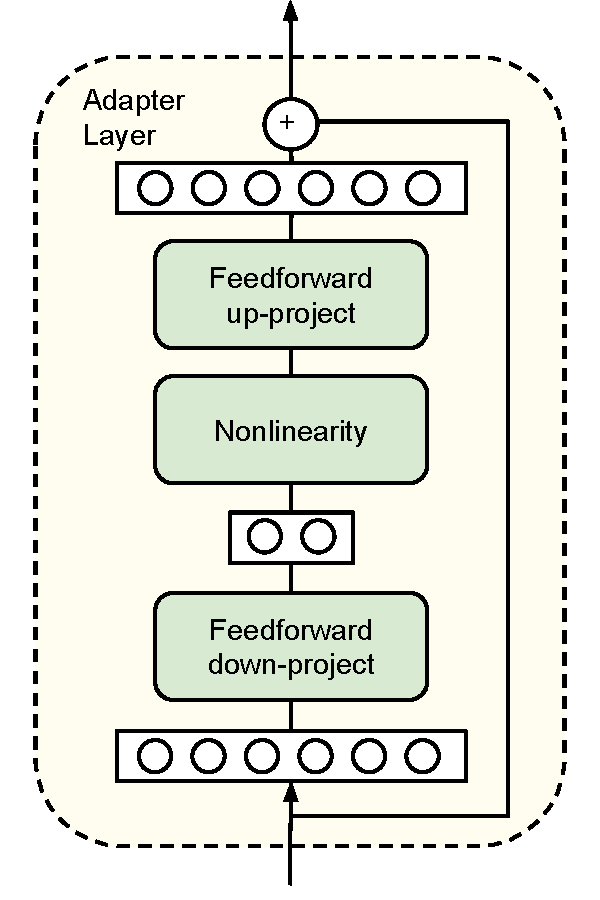
\includegraphics[width=\textwidth]{figs/lex_parsing/adapters/adapter_arch.pdf}
    \end{subfigure}%
    \begin{subfigure}[t]{0.5\textwidth}
        \centering
        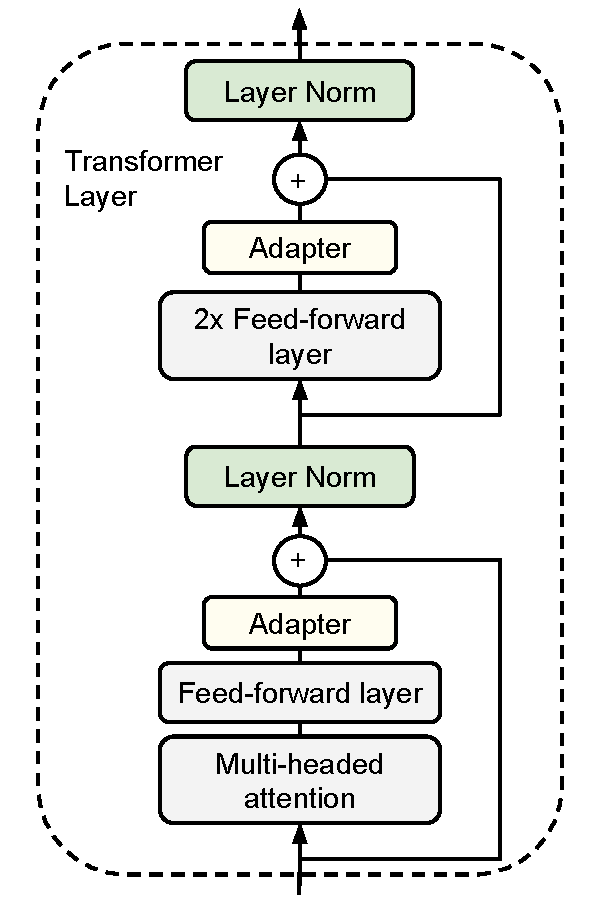
\includegraphics[width=\textwidth]{figs/lex_parsing/adapters/adapter_insertion.pdf}
        %\caption{加入適應器後的轉換器架構(圖取自\cite{rebuffi2018efficient})。}
    \end{subfigure}
    \caption{\textbf{左側}:適應器架構;\textbf{右側}:加入適應器後的轉換器架構(圖取自\cite{rebuffi2018efficient})。}
    \label{fig:adapter}
\end{figure}

適應器為雷氏(Sylvestre-Alvise Rebuffi)\cite{rebuffi2018efficient}所提出在影像領域的轉移學習方法,
後由何氏(Neil Houlsby)引進自然語言處理常用的轉換器模型\cite{houlsby2019parameter},
其指出當時自然語言處理的轉移學習方法多半使用大型預訓練轉換器模型進行全模型精細校正在目標任務上,
但何氏認為全模型精細校正需要調整模型中所有的參數,每種任務都會產生一個全新的模型,
太耗費儲存空間與計算資源,且大型預訓練轉換器模型已經含有大量句法語意等任務所需資訊,應不需要變動參數過多;
因此他提出固定原本的大型預訓練轉換器模型參數,但在被固定的模型層中加入具殘差網路性質的適應器,
模型只需為每個任務調整適應器少量的參數,任務間還是共享原本的大型預訓練轉換器模型參數,
而實驗數據也顯示,加入適應器的轉換器模型可以在所需調整的參數量遠低於全模型精細校正下,在目標任務中達成與其相似的表現。
其架構為一前饋層組成的兩層瓶頸網路(一層投射到較小維度,一層投射回原本維度),
再加上殘差連結(residual),置於轉換器中前饋層後、層\XNorm 之前的位置,細節可見圖\ref{fig:adapter}。
%其指出學習一通用特徵抽取器(universal feature extractor),
%然後在其後為每個任務接上一個任務專屬模組(task-specific module)做精細校正,
%這樣的方法雖然可以充分利用通用特徵抽取器的精緻特徵一次解決多個任務,但其各自任務的表現通常沒有專精單一任務來得好;
%因此他提出在通用特徵抽取器
%\input{figs/delex_parsing/adapters/adapter_ins.tex}

\section{實驗設置}

%\subsection{基準模型與元學習模型共同實驗設置}
\begin{table}[htbp]
    % \fontsize{8}{10}\selectfont
    \centering
    \begin{subtable}[t]{.4\textwidth}
        \begin{tabular}[t]{@{}lr@{}}
        \toprule
        超參數 & 值 \\
        \midrule
            依存標籤維度         & 256 \\
            依存邊維度           & 768 \\
            丟棄機率            & 0.5 \\
            BERT丟棄機率        & 0.2 \\
            BERT遮蔽機率        & 0.2 \\
            層丟棄機率          & 0.1 \\
            批次大小$b$         & 16 \\
            語言數$l$           & 10 \\
            訓練樣本數/回合        & 64000 \\
            訓練回合數          & 10 \\
            優化器              & Adam \\
            $\beta_1,\beta_2$  & 0.9, 0.9 \\
            權重衰減參數         & 0.01 \\
            基礎學習率          & $3e^{-4}$ \\
            最大梯度            & 5.0 \\
        \bottomrule
        \end{tabular}
        \caption{
            預訓練超參數。
        }
        \label{tab:pretrain_hparams}
    \end{subtable}
    \begin{subtable}[t]{.4\textwidth}
        \begin{tabular}[t]{@{}lr@{}}
        \toprule
        超參數 & 值 \\
        \midrule
            丟棄機率            & 0.5 \\
            BERT丟棄機率        & 0.2 \\
            BERT遮蔽機率        & 0.2 \\
            層丟棄機率          & 0.1 \\
            批次大小            & 16 \\
            訓練回合數          & 80 \\
            優化器              & Adam \\
            $\beta_1,\beta_2$  & 0.9, 0.99 \\
            權重衰減參數         & 0.01 \\
            基礎學習率          & $3e^{-4}$ \\
            最大梯度範數        & 5.0 \\
        \bottomrule
        \end{tabular}
        \caption{
            精細校正超參數。
        }
        \label{tab:finetune_hparams}
    \end{subtable}
    \caption{
        詞化依存句法剖析模型超參數一覽。
    }
    \label{tab:hparams}
\end{table}


% 本節的實驗設置基於\conll的實驗設置,但做了些微改變:
% 我們從\conll的53種訓練語言(73個訓練句法樹庫)中選取有官方驗證集(development set)的46種訓練語言(66個訓練句法樹庫)作爲訓練語言;見表\ref{tab:training_languages}。
% 預訓練完成後,我們分別對該模型進行\zeroshot及\finetune在預訓練中未見過的語言上。
%本節實驗在訓練語言與測試語言的切分與章節\ref{subsec:delex_depparse_setting}去詞化的依存句法剖析設置大致相同,不再贅述。
本節實驗設置與第\ref{sec:delex_depparse_setting}節去詞化的依存句法剖析設置大致相同,不再贅述。
% 而訓練方法部分,
% 在訓練時也均使用正確的斷句、斷詞,
% 惟測試時爲了與\conll相比,由於\conll連句法剖析之前的預處理(斷句、斷詞)也納入整體評分,
% 但研究重點在句法剖析而非預處理,
% 因此直接採用StanfordNLP的預處理系統\cite{qi-etal-2018-universal}\footnote{https://github.com/stanfordnlp/stanfordnlp}。

%孔氏\cite{kondratyuk-straka-2019-75}與烏氏\cite{ustun2020udapter}進行多語言訓練的方法,是將全部語言的句法樹庫接在一起、在一個小批次(batch)中混合多個句法樹庫訓練。
%這樣的做法可能會導致資料量大的語言取樣頻率過高;我們的方法則是每次更新從全部語言裡取樣$l$種語言,每種語言取樣$b$個句子,一個批次總共有$b \times l$個句子。
%不同於孔氏與烏氏,這樣的方法防止模型過度對資料充足語言的特性建模,但也可能使得資料不足語言的句子被過度取樣而產生過擬合的現象。

模型部份,本研究跟隨烏氏的做法,採用適應器模型\finetune $\mathrm{mBERT}$在依存句法剖析任務上。
除了優化器的學習率調整方法不同以外,大部分的超參數都與烏氏的設置一樣;見表\ref{tab:pretrain_hparams}。

其他設置均與章節\ref{sec:delex_depparse_setting}所述相同。

%\subsection{元學習實驗設置}

%對於\reptile與\fomaml,如無特別註明,外迴圈學習率(outer-loop learning rate)與內迴圈學習率(inner loop-learning rate)相同。
%\subsubsection{\zeroshot(Zero-shot Transfer)實驗設置}
%我們選取CoNLL 2018 Shared Task中只有訓練集而沒有發展集的語言作爲測試語言。


\finetune 的超參數請見表\ref{tab:finetune_hparams}。

% 由於選取的測試語言都沒有官方驗證集,在此說明從訓練集中分割出驗證集的方式:
% 對於訓練集少於100筆資料的語言(有Buryat、Kurmanji、Upper Sorbian、Kazakh、Armenian),以$k$摺交叉驗證(k-fold cross-validation)的方式
% 得到$k$個模型,並對這$k$個模型做模型集成(model ensemble)。對所有的實驗,我們設$k = 3$;
% 對於訓練集大於100筆資料的語言(有Irish、North Sami),則隨機切出$\frac{1}{8}$的訓練資料作為驗證資料。

\section{實驗結果}
% \subsection{\zeroshot(Zero-shot Transfer)}
% %\begin{figure}[h]
    \centering
    \includegraphics{figs/chapter3/dir_size_las_zs_multi-adapter-crf.pdf}
    \caption{方向性與數據量對基準模型\zeroshot的LAS的影響}
    \label{fig:dir-size-las-zs-multi-adapter-crf}
\end{figure}
% 基準模型進行\zeroshot的結果呈現於圖。%\ref{fig:dir-size-las-zs-multi-adapter-crf}。
% \iffalse
% \begin{table}[!ht]
    \fontsize{8}{10}\selectfont
    \begin{center}
    \setlength{\tabcolsep}{2pt}
    \begin{tabularx}{0.65\textwidth}{@{}l|lcccccccc@{}}
    \toprule
    Setting & Model                             &   bxr   &     kmr   &       hsb &        kk &    hy & ga    & sme   & average \\
    \midrule
    \multirow{ 1}{*}{Baseline} & \sc Stanford   &   13.49 &  \bf   24.15 &     22.97 &     26.25 &     32.70 &  \bf  70.34 &   \bf  70.99 &     27.27 \\
    \hline
    \multirow{ 7}{*}{ZS}
    & $\textsc{Multi}$ & 27.15 & 11.11 & 49.62 & 54.95 & 63.52 & 46.48 & 11.49 & 37.76 \\
    & $\textsc{Fomaml}$ & 26.98 & 11.52 & 48.65 & 53.04 & 62.18 & 46.74 & 11.80 & 37.27 \\
    & $\textsc{Reptile}$ & 27.26 & 11.55 & 49.40 & 53.85 & 62.80 & 47.08 & 11.75 & 37.67 \\
    & $\textsc{Multi\&Reptile}$ & 27.19 & 11.12 & 49.61 & 54.64 & 63.13 & 47.16 & 11.65 & 37.79 \\
    & $\textsc{Multi\&Fomaml}$ & 27.25 & 11.17 & 49.26 & 54.38 & 62.90 & 47.21 & 11.63 & 37.69 \\
    \hline
    \multirow{ 5}{*}{FT} &  \sc Multi                         &     26.37 &     14.86 & \bf 53.98 &     58.63 &     65.81 &     66.39 &     63.63 &     49.95 \\
    & \sc Reptile                       &     27.08 &     14.27 &     52.68 &     58.58 &     66.11 &     66.36 &     63.47 &     49.79 \\
    & $\textsc{Multi}^{\alpha}$              &     24.04 &     15.35 &     48.61 &     51.73 &     54.37 & \bf 67.21 &     63.55 &     46.40 \\
    & $\textsc{Reptile}^{\alpha}$            &     24.69 &     13.72 &     48.96 &     52.14 &     59.93 &     66.98 &     63.50 &     47.13 \\
    & $\textsc{M\&M}$                   & \bf 28.33 & \bf 17.14 &     53.61 & \bf 60.41 & \bf 66.41 &     66.60 & \bf 64.31 & \bf 50.97 \\
    \bottomrule
    \end{tabularx}
    \end{center}
    \caption{\label{table:las_all}
    Zero-shot (ZS) and fine-tuned (FT) test LAS scores of multi-task (\textsc{Multi}), Reptile (\textsc{Reptile}) averaging over seeds, ensemble of two multi-task and reptile models with different seeds ($\textsc{Multi}^{e}$, $\textsc{Reptile}^{e}$),  interpolation of two multi-task and reptile models with different seeds ($\textsc{Multi}^{\alpha}$, $\textsc{Reptile}^{\alpha}$), and interpolation of multi-task and Reptile models with the same random seed ($\textsc{M\&M}$). Our 
    }
\end{table}
% \fi
% \subsection{單語言\finetune(Monolingual Fine-tuning)}

%基準模型進行單語言\finetune的結果呈現於圖\ref{fig:dir-size-las-ft-multi}。從該圖可以發現,句法樹庫的大小幾乎決定了基準模型進行單語言\finetune在各種語言上的表現。

%\fomaml模型進行單語言\finetune的結果相對於基準模型的進步量呈現於圖\ref{fig:dir-size-las-ft-fomaml-to-multi}。從該圖可以發現,\fomaml主要在資料不足語言表現較基準模型稍佳,而在資料充足語言則差異不大。
%模型進行單語言的結果相對於基準模型的進步量呈現於圖\ref{fig:dir-size-las-ft-fomaml-to-multi}。從該圖可以發現,主要在資料不足語言表現較基準模型稍佳,而在資料充足語言則差異不大。

%\reptile模型進行單語言\finetune的結果相對於基準模型的進步量呈現於圖\ref{fig:dir-size-las-ft-reptile-to-multi}。從該圖可以發現,\reptile主要在資料不足語言表現較基準模型稍佳,而在資料充足語言則差異不大。

%\begin{figure}[h]
    \centering
    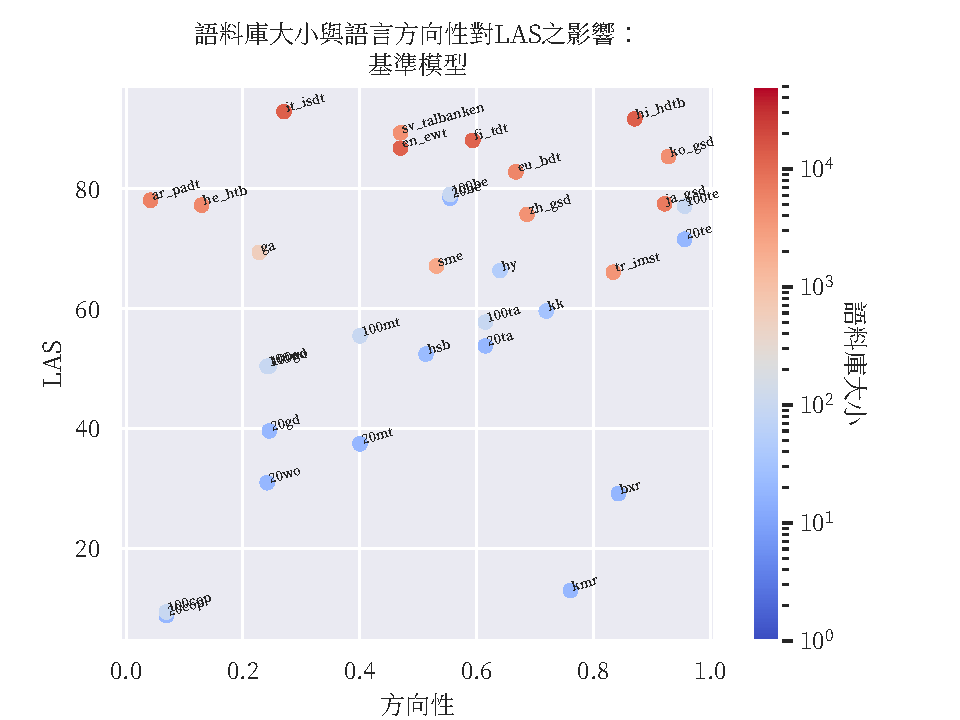
\includegraphics{figs/lex_parsing/dir_size_las_ft_multi.pdf}
    \caption{方向性與數據量對基準模型進行單語言\finetune後LAS的影響}
    \label{fig:dir-size-las-ft-multi}
\end{figure}

%\begin{figure}[h]
    \centering
    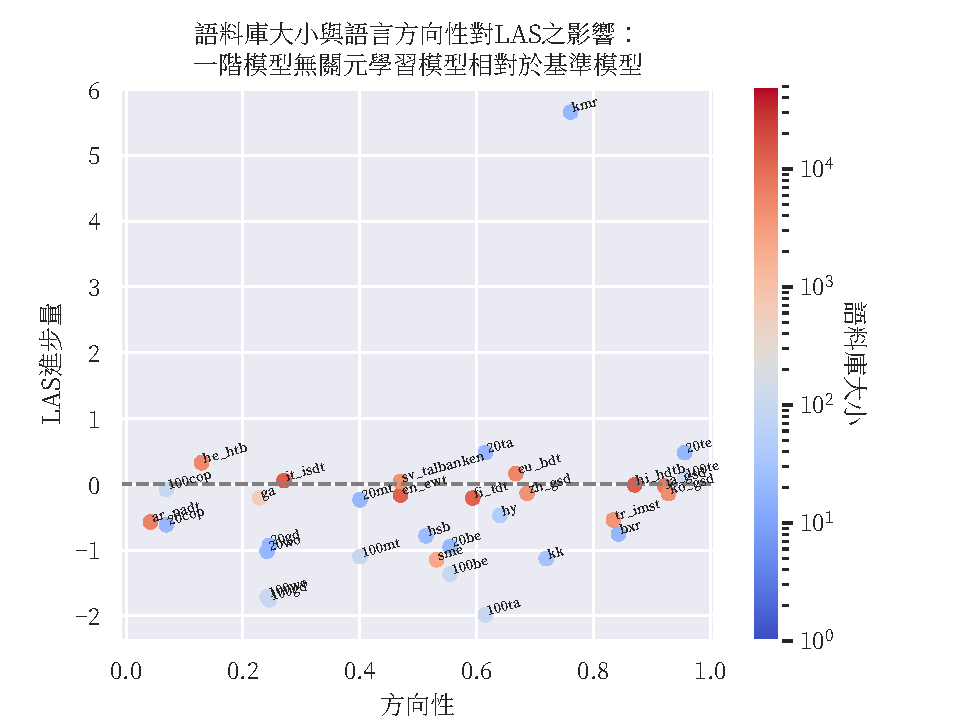
\includegraphics{figs/lex_parsing/dir_size_las_ft_fomaml-to-multi.pdf}
    \caption{方向性與句法樹庫大小對\fomaml模型相對於基準模型各自進行單語言\finetune後LAS之進步量的影響}
    \label{fig:dir-size-las-ft-fomaml-to-multi}
\end{figure}

%\begin{figure}[h]
    \centering
    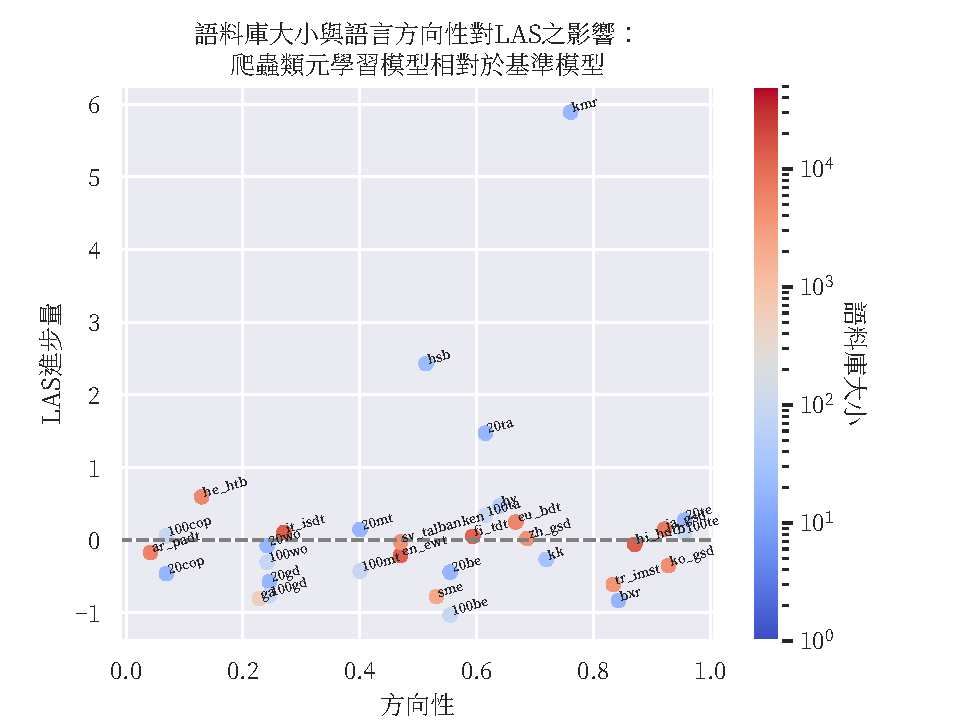
\includegraphics{figs/chapter3/dir_size_las_ft_reptile-to-multi.pdf}
    \caption{方向性與句法樹庫大小對\reptile 模型相對於基準模型各自進行單語言\finetune 後LAS之進步量的影響}
    \label{fig:dir-size-las-ft-reptile-to-multi}
\end{figure}
\begin{figure}[htbp]
    \centering
    \begin{subfigure}[t]{\textwidth}
        \centering
        \includegraphics[width=\textwidth]{figs/lex_parsing/linecharts/lex_train_langs.pdf}
    \end{subfigure}
    \vspace{-12pt}
    \begin{subfigure}[t]{\textwidth}
        \centering
        \includegraphics[width=\textwidth]{figs/lex_parsing/linecharts/lex_test_langs.pdf}
    \end{subfigure}
    \caption{依存句法剖析不同預訓練方法精細校正後的平均LAS折線圖。}
    \label{fig:lex_avg}
\end{figure}

\begin{figure}[htbp]
    \centering
    \begin{subfigure}[t]{0.8\textwidth}
        \centering
        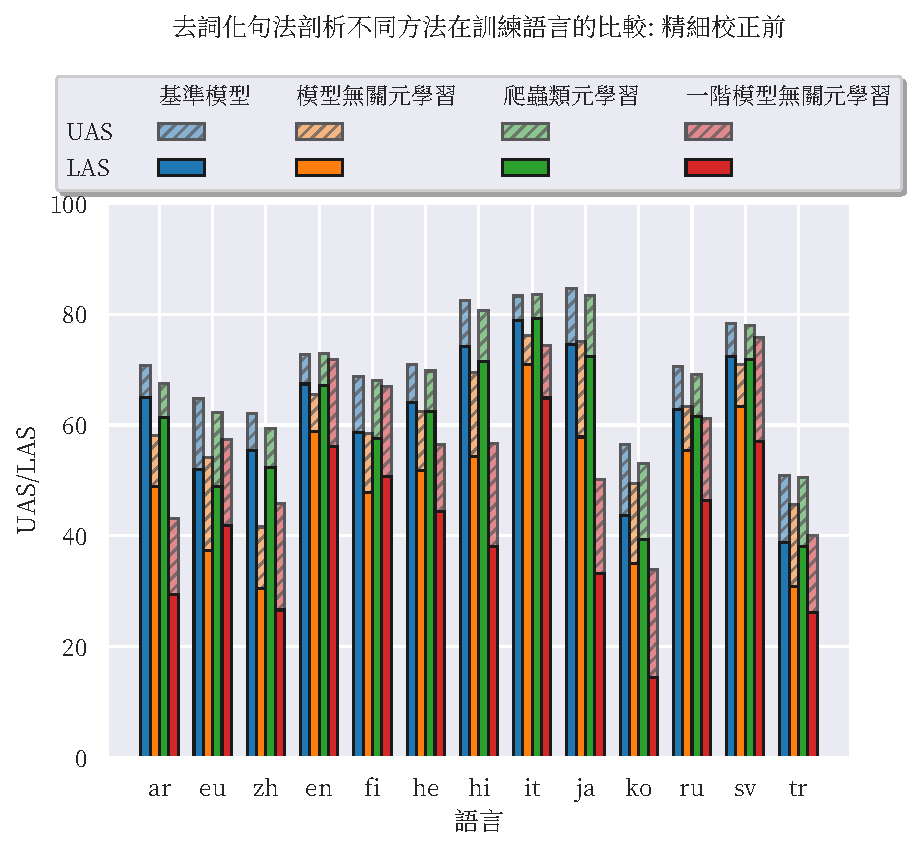
\includegraphics[width=\textwidth]{figs/lex_parsing/barplots/bar_zs_train_langs.pdf}
    \end{subfigure}
    \vspace{-12pt}
    \begin{subfigure}[t]{0.8\textwidth}
        \centering
        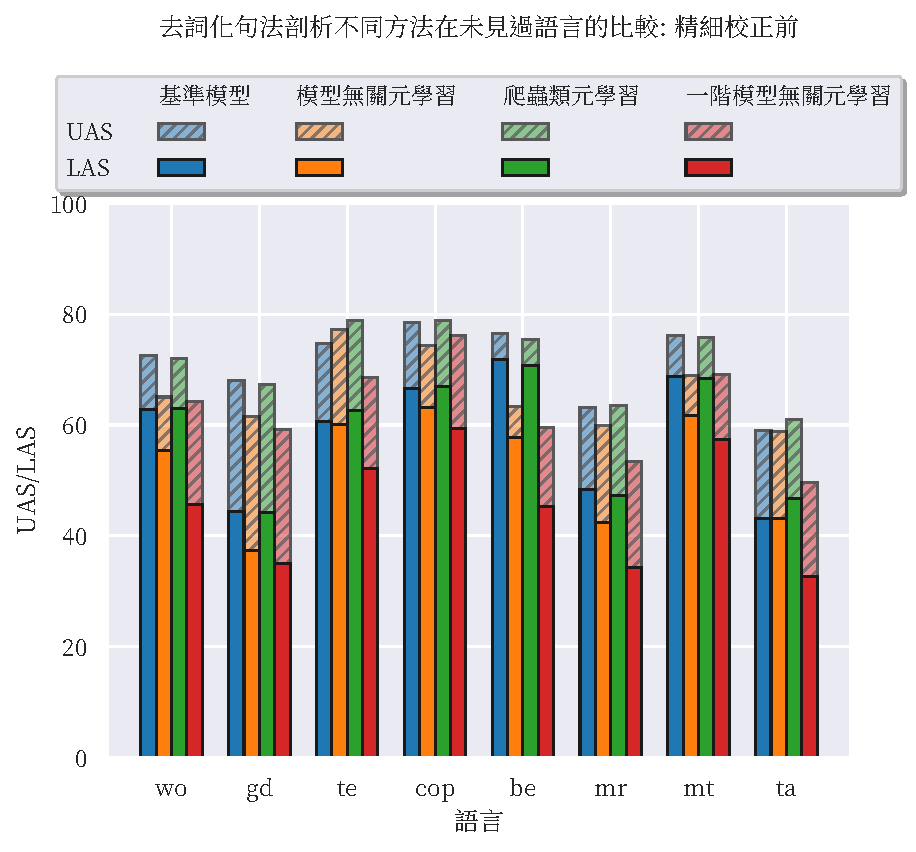
\includegraphics[width=\textwidth]{figs/lex_parsing/barplots/bar_zs_test_langs.pdf}
    \end{subfigure}
    \caption{依存句法剖析不同方法在各語言精細校正前的UAS/LAS長條圖。}
    \label{fig:lex_bar_zs}
\end{figure}
\begin{figure}[htbp]
    \centering
    \begin{subfigure}[t]{0.8\textwidth}
        \centering
        \includegraphics[width=\textwidth]{figs/lex_parsing/barplots/bar_constlr_one_step_train_langs.pdf}
    \end{subfigure}
    \vspace{-12pt}
    \begin{subfigure}[t]{0.8\textwidth}
        \centering
        \includegraphics[width=\textwidth]{figs/lex_parsing/barplots/bar_constlr_one_step_test_langs.pdf}
    \end{subfigure}
    \caption{依存句法剖析不同方法在各語言精細校正一步($\frac{1}{6}$回合)後的UAS/LAS長條圖。}
    \label{fig:lex_bar_one_step}
\end{figure}
\begin{figure}[htbp]
    \centering
    \begin{subfigure}[t]{0.8\textwidth}
        \centering
        \includegraphics[width=\textwidth]{figs/lex_parsing/barplots/bar_constlr_full_epoch_1_train_langs.pdf}
    \end{subfigure}
    \vspace{-12pt}
    \begin{subfigure}[t]{0.8\textwidth}
        \centering
        \includegraphics[width=\textwidth]{figs/lex_parsing/barplots/bar_constlr_full_epoch_1_test_langs.pdf}
    \end{subfigure}
    \caption{依存句法剖析不同方法在各語言精細校正一回合後的UAS/LAS長條圖。}
    \label{fig:lex_bar_full_epoch_1}
\end{figure}
\begin{figure}[htbp]
    \centering
    \begin{subfigure}[t]{0.8\textwidth}
        \centering
        \includegraphics[width=\textwidth]{figs/lex_parsing/barplots/bar_constlr_full_epoch_80_train_langs.pdf}
    \end{subfigure}
    \vspace{-12pt}
    \begin{subfigure}[t]{0.8\textwidth}
        \centering
        \includegraphics[width=\textwidth]{figs/lex_parsing/barplots/bar_constlr_full_epoch_80_test_langs.pdf}
    \end{subfigure}
    \caption{依存句法剖析不同方法在各語言精細校正八十回合後的UAS/LAS長條圖。}
    \label{fig:lex_bar_full_epoch_80}
\end{figure}

\begin{figure}[htbp]
    \centering
    \begin{subfigure}[t]{0.7\textwidth}
        \centering
        \includegraphics[width=\textwidth]{figs/lex_parsing/dir_scatterplots/zs_train_langs.pdf}
    \end{subfigure}
    \vspace{-12pt}
    \begin{subfigure}[t]{0.7\textwidth}
        \centering
        \includegraphics[width=\textwidth]{figs/lex_parsing/dir_scatterplots/zs_test_langs.pdf}
    \end{subfigure}
    \caption{依存句法剖析不同方法在各語言精細校正前的方向性分佈。}
    \label{fig:lex_dir_scatter_zs}
\end{figure}
\begin{figure}[htbp]
    \centering
    \begin{subfigure}[t]{0.7\textwidth}
        \centering
        \includegraphics[width=\textwidth]{figs/lex_parsing/dir_scatterplots/constlr_one_step_train_langs.pdf}
    \end{subfigure}
    \vspace{-12pt}
    \begin{subfigure}[t]{0.7\textwidth}
        \centering
        \includegraphics[width=\textwidth]{figs/lex_parsing/dir_scatterplots/constlr_one_step_test_langs.pdf}
    \end{subfigure}
    \caption{依存句法剖析不同方法在各語言精細校正一步($\frac{1}{6}$回合)後的方向性分佈。}
    \label{fig:lex_dir_scatter_one_step}
\end{figure}
\begin{figure}[htbp]
    \centering
    \begin{subfigure}[t]{0.7\textwidth}
        \centering
        \includegraphics[width=\textwidth]{figs/lex_parsing/dir_scatterplots/constlr_full_epoch_1_train_langs.pdf}
    \end{subfigure}
    \vspace{-12pt}
    \begin{subfigure}[t]{0.7\textwidth}
        \centering
        \includegraphics[width=\textwidth]{figs/lex_parsing/dir_scatterplots/constlr_full_epoch_1_test_langs.pdf}
    \end{subfigure}
    \caption{依存句法剖析不同方法在各語言精細校正一回合後的方向性分佈。}
    \label{fig:lex_dir_scatter_full_epoch_1}
\end{figure}
\begin{figure}[htbp]
    \centering
    \begin{subfigure}[t]{0.7\textwidth}
        \centering
        \includegraphics[width=\textwidth]{figs/lex_parsing/dir_scatterplots/constlr_full_epoch_80_train_langs.pdf}
    \end{subfigure}
    \vspace{-12pt}
    \begin{subfigure}[t]{0.7\textwidth}
        \centering
        \includegraphics[width=\textwidth]{figs/lex_parsing/dir_scatterplots/constlr_full_epoch_80_test_langs.pdf}
    \end{subfigure}
    \caption{依存句法剖析不同方法在各語言精細校正八十回合後的方向性分佈。}
    \label{fig:lex_dir_scatter_full_epoch_80}
\end{figure}
